\documentclass[conference]{IEEEtran}
\IEEEoverridecommandlockouts
% The preceding line is only needed to identify funding in the first footnote. If that is unneeded, please comment it out.
\usepackage[utf8]{inputenc}
\usepackage{amsmath, amssymb, amsfonts}
\usepackage{float, graphicx, textcomp}
\usepackage{cite, listings, pdfpages, comment, fancyhdr, subcaption, tikz}
\usepackage[margin=0.8in]{geometry}
\usepackage[english]{babel}
\usepackage{xcolor}
\usepackage{enumerate}% http://ctan.org/pkg/enumerate
\usepackage{booktabs}
\usepackage[linesnumbered,ruled,vlined]{algorithm2e}
\usepackage{hyperref}
\hypersetup{colorlinks=true, linkcolor=blue, citecolor=blue, urlcolor=blue}

\def\BibTeX{{\rm B\kern-.05em{\sc i\kern-.025em b}\kern-.08em
    T\kern-.1667em\lower.7ex\hbox{E}\kern-.125emX}}

%% Shorthands used throughout
\newcommand{\cfrp}{CFR$^+$}
\newcommand{\pcfrp}{PCFR$^+$}
\newcommand{\ours}{LAD-CFR$^+$}
\newcommand{\mix}{MIX-CFR}
\newcommand{\pos}[1]{\left[#1\right]^{+}}

\begin{document}

\title{Locally Adaptive Regret Updates for Faster Equilibrium Finding in Imperfect-Information Games}

\author{\IEEEauthorblockN{Sadiqah Mushtaq}
\IEEEauthorblockA{\textit{Oregon State University}\\
Corvallis, Oregon, USA \\
mushtasa@oregonstate.edu}
\and
\IEEEauthorblockN{Umna Khawaja}
\IEEEauthorblockA{\textit{Oregon State University}\\
Corvallis, Oregon, USA \\
khawajau@oregonstate.edu}
\and
\IEEEauthorblockN{Kagan Tumer}
\IEEEauthorblockA{\textit{Oregon State University}\\
Corvallis, Oregon, USA \\
Kagan.Tumer@oregonstate.edu}
}

\maketitle
\pagenumbering{arabic}

\begin{abstract}
Many multiagent settings, such as poker, negotiation and security planning, require agents to
make decisions without knowing what their opponents know.
Strong strategies for these imperfect-information games can be learned through repeated
self-play, in which agents learn from their regret, but every round traverses the entire game
tree, so the number of iterations needed largely determines which games can be solved.
Counterfactual Regret Minimization (CFR) is the leading approach, and its variants speed it up
by changing how regrets are accumulated, with recent ones even adapting these choices
automatically.
However, these methods still apply the same update rule at every information set, even
though regret changes rapidly at some and has already stabilized at others.
In this work, we study two ways of adapting the update locally: \ours{}, in which each
information set chooses its own regret discount based on how volatile its recent regrets are,
and \mix{}, in which each information set learns online which of \cfrp{}, Discounted CFR and
Predictive \cfrp{} to follow, while remaining a no-regret method.
On five games, adapting only the discount gives modest gains, whereas \mix{}, without any
tuning, is the best or close to the best method on every game, while each existing variant
falls far behind on at least one.
\end{abstract}

\begin{IEEEkeywords}
Multiagent Systems, Game Theory, Counterfactual Regret Minimization, Imperfect-Information
Games, Nash Equilibrium
\end{IEEEkeywords}


\section{Introduction}

% Q1: What is the problem and why do I care?
Solving imperfect-information games is a major challenge in multiagent systems, with
applications from poker to security~\cite{tambe2011security}, where agents
have to make strategic decisions without being able to observe the complete state of the
environment or the private information available to their opponents. A representative example
of this is poker, where players have to choose actions based on their private cards, public
information, the betting history, and their beliefs about other players' hidden
cards~\cite{bowling2015heads, moravcik2017deepstack, brown2018superhuman, brown2019superhuman}. A main
goal in these settings is to calculate strategies that are difficult for the opponent to
exploit. A widely used approach for this is Counterfactual Regret Minimization
(CFR)~\cite{zinkevich2007regret}, since it iteratively improves strategies by minimizing the
regret over possible actions at every information set. However, convergence may require many
iterations, making computational efficiency an important concern when solving larger
games~\cite{tammelin2015solving}.

% Q2: Why is it important/difficult?
It is difficult to solve imperfect-information games, since an agent has to account for
uncertainty regarding the underlying game state while also reasoning about the strategic
responses of other agents. Unlike in perfect-information games, an agent cannot select actions
based on a fully observed state. It must, instead, learn a strategy that will perform well
across the multiple possible states that are consistent with its observations. CFR addresses
this challenge by decomposing regret minimization across information sets; however, the amount
and pattern of regret may vary substantially across these sets. Some information sets might
exhibit rapidly changing regret, while others might have relatively stable regret. Applying the
same update procedure throughout the game might therefore fail to exploit the differences in
local learning dynamics.

% Q3: What has been done already in this problem area?
Several methods have already improved the efficiency of regret minimization. CFR introduced an
iterative framework for minimizing counterfactual regret and established convergence guarantees
for the average strategy in two-player zero-sum games~\cite{zinkevich2007regret}. \cfrp{} then
improved practical convergence by using regret matching$^+$, alternating player updates, and
linear averaging~\cite{tammelin2015solving}. Discounted CFR introduced discounting schemes that
reduce the influence of earlier iterations and can accelerate convergence~\cite{brown2019solving}.
Predictive \cfrp{} further explores the use of predicted regret updates to improve game-solving
speed~\cite{farina2021faster}, and PDCFR$^+$ combines prediction with
discounting~\cite{xu2024minimizing}. More recent methods also adapt these choices automatically:
DDCFR learns its discounting with reinforcement learning~\cite{xu2024dynamic}, hyperparameter
schedules change the discounting over time~\cite{zhang2026faster}, VAD-CFR adjusts discounting
using a single, game-wide measure of regret volatility~\cite{li2026discovering}, and APCFR$^+$
adapts the size of its predicted regret updates separately at each information
set~\cite{meng2025faster}. Together, these methods demonstrate that how regret is modified,
accumulated, weighted, and updated can drastically affect convergence.

% Q4: What particular problem remains unsolved?
Despite all of these advances, the question of whether the discounting of past regret should
adapt to the recent dynamics of individual information sets remains worth investigating. It is
especially worth noting that a fixed discounting procedure might not respond equally well to
information sets whose regrets are changing rapidly and to those whose regrets have stabilized.
Even though existing approaches have modified regret updates, used predictive information, or
adapted their discounting for the game as a whole, this work investigates a complementary
approach: adapting the regret update locally according to recent regret dynamics, and whether
this improves convergence. An open empirical question is under which conditions
this would be most beneficial.

% Q5: How did you solve it?
In this work, we present two methods. The first, Locally Adaptive Discounted \cfrp{} (\ours{}),
is a modification of \cfrp{} that uses the recent regret history at individual information
sets to determine how much past regret should be kept. Instead of using an identical discount
at each information set, it adjusts the discount according to the observed local regret
dynamics. The second, \mix{}, goes further: each information set runs \cfrp{}, Discounted CFR
and Predictive \cfrp{} side by side, and a small regret-matching learner at that information
set learns which of them to follow. Both algorithms are implemented using
OpenSpiel~\cite{lanctot2019openspiel} and evaluated on Kuhn Poker~\cite{kuhn1950simplified} and
Leduc Poker~\cite{southey2005bayes}, two imperfect-information poker games that provide
increasingly complex test environments, and on three further games, two sizes of Liar's dice
and Goofspiel, to test whether the results transfer beyond poker.

% Q6: What is cool about your approach?
Our main motivation behind \ours{} is that different parts of a game might exhibit different
learning dynamics. By incorporating the local regret history into the update procedure, the
method aims to discount past regret more strongly at information sets where the regret is
changing greatly, so that they respond quickly, while keeping the regret history where it has
stabilized. \mix{} applies the same idea to the choice of update rule itself: since no existing variant
is fastest on every game, each information set can follow whichever rule works best there,
and regret matching over the rules keeps the method no-regret without any parameter to tune.
In contrast to a uniform modification applied throughout the game, our approach explicitly
examines the variation in regret behavior across information sets.

% Q7: What were your key results?
To evaluate our methods, we compare them against \cfrp{}, Discounted CFR, and Predictive
\cfrp{}. As a first step, we reproduce the CFR versus \cfrp{} comparison on Kuhn and Leduc
Poker using OpenSpiel, whose CFR implementation uses alternating updates. \cfrp{} reaches
roughly $12\times$ lower exploitability than CFR on Kuhn Poker after 2000 iterations and
$46\times$ lower on Leduc Poker after 1000 iterations. Our main measure is exploitability,
which is how much a best-responding opponent could win against the agents' average strategy,
as a function of the number of iterations. We also compare each method with an otherwise
identical version that adapts at the level of the whole game, to test whether adapting locally
is what makes the difference. We find that no existing variant is fastest on every game:
Predictive \cfrp{} is best on Kuhn Poker but worst on Leduc Poker. \ours{} improves on \cfrp{}
with the same averaging on four of five games, and its local version beats its game-wide
version on all five, but its gains are modest. \mix{}, without any tuning, is the best method
on Kuhn and Leduc Poker and within $1.13\times$ of the best on the other three games, and on
two games it outperforms every rule it combines.

% Q8: What are the contributions of this paper?
The main contributions of this work are:
\begin{enumerate}
  \item We develop an adaptive regret-update approach, \ours{}, that incorporates local
        regret dynamics into \cfrp{} by adapting how much past regret each information set
        keeps.
  \item We develop \mix{}, which selects among existing CFR update rules separately at each
        information set, and show that it remains no-regret.
  \item We establish an experimental comparison of our methods against established
        regret-minimization baselines on Kuhn Poker, Leduc Poker, Liar's dice and Goofspiel.
  \item We investigate the conditions under which local adaptation improves
        convergence, including differences between game environments and the effects of
        individual components through ablation studies.
\end{enumerate}
The results provide evidence regarding the potential benefits and limitations of adapting
regret updates at the information-set level.


\section{Background}

This section defines the problem setting (Sections~\ref{sec:efg}--\ref{sec:domains}), the
foundations our method builds on (Section~\ref{sec:cfr}), and the existing approaches to
speeding up CFR (Section~\ref{sec:variants}).

\subsection{Extensive-Form Games and Nash Equilibrium}
\label{sec:efg}

We model the problem as a finite \emph{extensive-form game} with imperfect
information~\cite{shoham2008multiagent}. Players in a set $N$ take turns acting, with a special
\emph{chance} player representing random events such as card deals. A \emph{history} $h$ is a
sequence of actions from the start of the game, $Z$ is the set of terminal histories, and
$u_i(z)$ is player $i$'s payoff at $z \in Z$. Histories that player $i$ cannot distinguish,
because they differ only in information hidden from $i$, are grouped into an \emph{information
set} $I \in \mathcal{I}_i$. The actions $A(I)$ available are the same at every history in $I$.

A \emph{strategy} $\sigma_i$ assigns a probability distribution $\sigma_i(I,\cdot)$ over $A(I)$
to every information set of player $i$, and a \emph{strategy profile} $\sigma$ contains one
strategy per player. We write $\pi^\sigma(h)$ for the probability of reaching $h$ under
$\sigma$, and $\pi^\sigma_{-i}(h)$ for the part of that probability contributed by chance and
all players other than $i$. The expected payoff is $u_i(\sigma) = \sum_{z\in Z}\pi^\sigma(z)\,
u_i(z)$.

A profile is a \emph{Nash equilibrium} if no player can improve its payoff by unilaterally
changing its strategy. In two-player zero-sum games ($u_1 = -u_2$), we measure distance from
equilibrium with \emph{exploitability},
\begin{equation}
  e(\sigma) = \frac{1}{2}\sum_{i\in\{1,2\}}\Big(\max_{\sigma_i'} u_i(\sigma_i',\sigma_{-i})
  - u_i(\sigma)\Big),
  \label{eq:expl}
\end{equation}
the average amount that a best-responding opponent could gain. Exploitability is zero exactly
at a Nash equilibrium. Exploitability is computed exactly by a best-response tree traversal, and is the
standard metric for comparing CFR variants~\cite{tammelin2015solving, brown2019solving}.

\subsection{Problem Domains}
\label{sec:domains}

We evaluate on two standard poker benchmarks small enough for exploitability to be computed
exactly.

\emph{Kuhn poker}~\cite{kuhn1950simplified} uses a three-card deck (Jack, Queen, King). Each of
two players antes one chip and receives one private card, followed by a single betting round
in which players may check, bet one chip, call or fold. If no one folds, the higher card wins. The game has 12 information sets, and its equilibria are known in
closed form, which makes it a useful correctness check.

\emph{Leduc poker}~\cite{southey2005bayes} uses a six-card deck containing two suits of Jack,
Queen and King. Each player antes one chip and receives one private card. After a first betting
round with bets of two chips, one public card is revealed, followed by a second round with bets
of four chips, with at most two raises per round. A player whose private card pairs the public
card wins; otherwise the higher card wins. Leduc poker adds two features that make full
Texas hold'em hard, multiple betting rounds and shared public information, while having only
936 information sets.

Both games are provided by OpenSpiel~\cite{lanctot2019openspiel}, an open-source framework that
implements the game rules, tabular policies, CFR and \cfrp{}, and exact exploitability.
OpenSpiel also provides three-player versions of both games.

\subsection{Regret Minimization and CFR}
\label{sec:cfr}

\emph{Regret} measures how much better an agent would have done had it always played a fixed
action instead of its actual sequence of strategies. An algorithm is \emph{no-regret} if its
average regret goes to zero. A central result connects learning to equilibrium: if both players
of a two-player zero-sum game have average regret at most $\epsilon$ after $T$ iterations of
self-play, their \emph{average} strategies form a $2\epsilon$-Nash
equilibrium~\cite{zinkevich2007regret}. \emph{Regret matching}~\cite{hart2000simple} is a
simple no-regret algorithm that plays each action in proportion to its positive cumulative
regret $R^T(a)$:
\begin{equation}
  \sigma^{T+1}(a) = \frac{\pos{R^T(a)}}{\sum_{b}\pos{R^T(b)}},
  \label{eq:rm}
\end{equation}
choosing uniformly at random if no regret is positive.

\emph{Counterfactual Regret Minimization}~\cite{zinkevich2007regret} applies regret matching
independently at every information set. The \emph{counterfactual value} of information set
$I \in \mathcal{I}_i$ is player $i$'s expected payoff from $I$, weighted by the probability
that chance and the opponents reach it:
\begin{equation}
  v_i^\sigma(I) = \sum_{h\in I}\sum_{z\in Z,\,h\sqsubseteq z}
  \pi^\sigma_{-i}(h)\,\pi^\sigma(h,z)\,u_i(z),
\end{equation}
where $\pi^\sigma(h,z)$ is the probability of reaching $z$ from $h$. Writing $v_i^\sigma(I,a)$
for the same value when $i$ plays $a$ at $I$, the \emph{instantaneous counterfactual regret}
at iteration $t$ is
\begin{equation}
  r^t_I(a) = v_i^{\sigma^t}(I,a) - v_i^{\sigma^t}(I).
  \label{eq:instregret}
\end{equation}
CFR accumulates $R^t_I(a) = R^{t-1}_I(a) + r^t_I(a)$ and picks the next strategy at each
information set with~\eqref{eq:rm}. Zinkevich et al.\ showed that the overall regret is bounded
by the sum of these local regrets, so the average strategy converges to a Nash equilibrium at a
rate of $O(1/\sqrt{T})$ in two-player zero-sum games.

In \emph{predictive} no-regret learning, the learner acts on a guess of its next loss, so its
regret depends on how wrong its guesses are rather than on the size of the losses, which can
speed up learning in games considerably~\cite{rakhlin2013optimization, syrgkanis2015fast}.

\subsection{Faster CFR Variants}
\label{sec:variants}

\textbf{\cfrp{}}~\cite{tammelin2015solving} makes three changes to CFR. First,
\emph{regret matching$^+$} keeps cumulative regrets non-negative,
\begin{equation}
  R^t_I(a) = \pos{R^{t-1}_I(a) + r^t_I(a)},
  \label{eq:rmplus}
\end{equation}
so an action that becomes good is played immediately. It also updates players in alternation
and weights iteration $t$ by $t$ in the average strategy, and was used to essentially solve
heads-up limit Texas hold'em~\cite{bowling2015heads}.

\textbf{Discounted CFR}~\cite{brown2019solving} multiplies accumulated positive regrets by
$t^\alpha/(t^\alpha+1)$, negative regrets by $t^\beta/(t^\beta+1)$, and average-strategy
contributions by $(t/(t+1))^\gamma$, with $\alpha=3/2$, $\beta=0$, $\gamma=2$ consistently
outperforming \cfrp{} in their experiments. These factors depend only on $t$ and are identical at every information
set.

\textbf{Predictive \cfrp{}}~\cite{farina2021faster} keeps update~\eqref{eq:rmplus} but plays
from the cumulative regret plus a prediction of the next instantaneous regret,
\begin{equation}
  \sigma^{t+1}_I(a) \propto \pos{R^t_I(a) + r^t_I(a)},
  \label{eq:pcfr}
\end{equation}
and \textbf{PDCFR$^+$}~\cite{xu2024minimizing} combines this prediction with DCFR-style
discounting.

Recent methods make these choices adaptive. \textbf{DDCFR}~\cite{xu2024dynamic} adjusts DCFR's
discount parameters during a run with a policy trained by reinforcement learning, while
\textbf{hyperparameter schedules}~\cite{zhang2026faster} change them as fixed functions of $t$.
\textbf{APCFR$^+$}~\cite{meng2025faster} scales the prediction in~\eqref{eq:pcfr} separately at
each information set, trusting it less where past predictions were inaccurate. \textbf{VAD-CFR},
found by an LLM-driven search over CFR variants~\cite{li2026discovering}, adjusts the discount
using a moving average of regret magnitude, although its authors found this component mattered
little on unseen games.

As Table~\ref{tab:prior} shows, the prediction has been adapted per information set, but the
discount on past regret only globally; \ours{} addresses this gap.

\begin{table}[t]
\centering
\caption{What existing CFR variants vary during a run, how, and at what scope.}
\label{tab:prior}
\setlength{\tabcolsep}{3pt}
\begin{tabular}{@{}llll@{}}
\toprule
\textbf{Method} & \textbf{Varies} & \textbf{How} & \textbf{Scope} \\
\midrule
\cfrp{}~\cite{tammelin2015solving}         & ---        & fixed         & --- \\
DCFR~\cite{brown2019solving}               & discount   & fixed in $t$  & global \\
\pcfrp{}~\cite{farina2021faster}           & ---        & fixed         & --- \\
PDCFR$^+$~\cite{xu2024minimizing}          & discount   & fixed in $t$  & global \\
DDCFR~\cite{xu2024dynamic}                 & discount   & learned (RL)  & global \\
HS~\cite{zhang2026faster}                  & discount   & schedule      & global \\
APCFR$^+$~\cite{meng2025faster}            & prediction & online        & per info.\ set \\
VAD-CFR~\cite{li2026discovering}           & discount   & online        & global \\
\midrule
\textbf{\ours{} (ours)}                    & \textbf{discount} & \textbf{online} & \textbf{per info.\ set} \\
\bottomrule
\end{tabular}
\end{table}


\section{Method}
\label{sec:method}

We study two ways of adapting the regret update to the local dynamics of each information set.
Both keep the rest of \cfrp{} unchanged: alternating updates, a full tree traversal per
iteration, and counterfactual values computed exactly as in Section~\ref{sec:cfr}.

\subsection{\ours{}: Locally Adaptive Discounting}
\label{sec:lad}

\ours{} gives every information set its own discount on past regret,
\begin{equation}
  Q^t_I = \pos{\gamma_I\, Q^{t-1}_I + r^t_I}, \qquad
  \gamma_I = 1 - \big(1 - d_{t-1}\big)\, v_I,
  \label{eq:lad}
\end{equation}
where $d_t = t^{\alpha}/(t^{\alpha}+1)$ is the DCFR discount with $\alpha = 3/2$. The
\emph{volatility} $v_I \in [0,1]$ measures how much the instantaneous regret of $I$ changes
between the iterations at which $I$ is reached,
\begin{equation}
  v_I = \frac{\operatorname{EMA}\,\lVert r^t_I - r^{t'}_I\rVert^2}
             {2\,\operatorname{EMA}\big(\lVert r^t_I\rVert^2 + \lVert r^{t'}_I\rVert^2\big)},
  \label{eq:vol}
\end{equation}
where $t'$ is the previous iteration with non-zero regret at $I$ and EMA is an exponential
moving average with memory $\lambda$. If the regrets keep pointing in the same direction,
$v_I \approx 0$ and~\eqref{eq:lad} reduces to \cfrp{}; if they flip sign every iteration,
$v_I \approx 1$ and $I$ is discounted like DCFR. A \emph{global} variant uses one volatility
computed from the regrets of all information sets.

\subsection{MIX-CFR: Locally Selecting the Update Rule}
\label{sec:mix}

\begin{algorithm}[t]
\caption{MIX-CFR update at information set $I$}
\label{alg:mix}
\SetKwInOut{Input}{Input}
\Input{counterfactual regrets $r^t_I$ of the played strategy $\sigma^t_I$}
\For{each expert $k \in \{\text{\cfrp{}}, \text{DCFR}, \text{\pcfrp{}}\}$}{
  $g_k \leftarrow \langle \sigma^t_{I,k}, r^t_I\rangle$ \tcp*{gain of $k$ over the mixture}
  update expert $k$ with its own regret $r^t_I - g_k\mathbf{1}$ and get $\sigma^{t+1}_{I,k}$\;
}
$W_I \leftarrow \pos{W_I + g}$ \tcp*{regret matching$^+$ over experts}
$w \leftarrow W_I / \sum_k W_{I,k}$ (uniform if $W_I = 0$)\;
$\sigma^{t+1}_I \leftarrow \sum_k w_k\, \sigma^{t+1}_{I,k}$\;
\end{algorithm}

No single fixed update rule is best on every game (Section~\ref{sec:results}), so MIX-CFR lets
each information set choose among existing rules online. Every information set runs three local
regret minimizers, or \emph{experts}, side by side: regret matching$^+$ (\cfrp{}), discounted
regret matching with DCFR's $\alpha=3/2$, $\beta=0$ (DCFR), and predictive regret
matching$^+$ (\pcfrp{}). A small meta learner at the same information set plays a mixture of
their strategies and moves weight toward the expert whose strategy would have earned more there
(Algorithm~\ref{alg:mix}). Because the played strategy satisfies
$\langle\sigma^t_I, r^t_I\rangle = 0$, the gain $g_k$ is exactly how much better expert $k$'s
strategy would have done than the mixture. The meta learner is itself regret
matching$^+$, so MIX-CFR has no learning rate or other parameter to tune. In the global
variant, a single meta learner per player receives the gains summed over all of that player's
information sets.

The decomposition behind Algorithm~\ref{alg:mix} also gives a guarantee. Writing $v$ for the
counterfactual action values at $I$, the regret of the mixture splits as
$r^t_I(a) = \big(v(a) - \langle\sigma^t_{I,k}, v\rangle\big) + g_k$ for every expert $k$, so
summing over iterations,
\begin{equation}
  \max_a R^T_I(a) \;\le\; \min_k \Big( \max_a R^T_{I,k}(a) + G^T_{I,k} \Big),
  \label{eq:mixbound}
\end{equation}
where $R^T_{I,k}$ is expert $k$'s own cumulative regret on the observed values and
$G^T_{I,k} = \sum_t g^t_k$ is the regret of the meta learner with respect to expert $k$. Regret
matching$^+$ keeps both $G^T_{I,k}$ and the regret of the \cfrp{} expert in
$O(\sqrt{T})$~\cite{tammelin2015solving}, so the local regret of MIX-CFR is $O(\sqrt{T})$
regardless of how the other experts behave, and by the CFR decomposition the uniform average
strategy converges to a Nash equilibrium in two-player zero-sum
games~\cite{zinkevich2007regret}. Bound~\eqref{eq:mixbound} also shows that, at each information
set separately, MIX-CFR is never much worse than the best of its experts. This is an instance of
composing regret minimizers~\cite{farina2019regret}. As with \pcfrp{} and DCFR, our experiments
use alternating updates and a $t^2$-weighted average strategy, to which this uniform-average
guarantee does not directly apply.


\section{Experimental Setup}
\label{sec:setup}

All methods are implemented in Python on top of OpenSpiel's tabular CFR
solver~\cite{lanctot2019openspiel}. \cfrp{} and DCFR are OpenSpiel's implementations, and
\pcfrp{}, \ours{} and MIX-CFR are subclasses of the same solver that change only the regret
update and the strategy computation. As correctness checks, \ours{} with $v_I$ fixed to $0$
reproduces OpenSpiel's \cfrp{} exactly, and MIX-CFR with a single expert reproduces \cfrp{}
and our \pcfrp{} up to floating-point rounding (maximum difference below $10^{-13}$).

\textbf{Games.} We use the five two-player zero-sum games in Table~\ref{tab:games}. Kuhn and
Leduc poker (Section~\ref{sec:domains}) are the original benchmarks. Liar's dice and
Goofspiel, both standard CFR benchmarks~\cite{lanctot2009monte}, were added to test whether
the conclusions transfer beyond poker. In Liar's dice each player privately rolls one die, and
players alternately make increasing claims about the dice of both players until one calls the
other a liar. In Goofspiel, players simultaneously bid cards from their hands to win prize
cards revealed in descending order, without seeing the opponent's bids.

\begin{table}[t]
\centering
\caption{Games used in the experiments (all from OpenSpiel).}
\label{tab:games}
\begin{tabular}{@{}lrr@{}}
\toprule
\textbf{Game} & \textbf{Info.\ sets} & \textbf{Iterations} \\
\midrule
Kuhn poker                  & 12    & 2000 \\
Leduc poker                 & 936   & 1000 \\
Liar's dice, 3 faces        & 192   & 1000 \\
Liar's dice, 4 faces        & 1024  & 1000 \\
Goofspiel, 4 cards          & 162   & 1000 \\
\bottomrule
\end{tabular}
\end{table}

\textbf{Methods.} We compare \cfrp{}, DCFR ($\alpha=3/2$, $\beta=0$, $\gamma=2$) and \pcfrp{}
($t^2$ averaging, as in~\cite{farina2021faster}) against \ours{} and MIX-CFR, each in a
local and a global version. \ours{} uses $\lambda = 0.99$ and $t^2$ averaging. These two
settings were selected from about 40 configurations evaluated on Kuhn and Leduc poker, and
were then fixed for the other three games. MIX-CFR uses no tuned parameters, and its experts
use their default settings. In the ablations, we remove one expert at a time and replace the
meta learner by its predictive version.

\textbf{Metric.} We report the exploitability~\eqref{eq:expl} of the average strategy, computed
exactly by OpenSpiel, at 30 log-spaced iterations. All methods traverse the full tree and are
deterministic, so each configuration is run once.


\section{Results}
\label{sec:results}

\begin{figure*}[t]
\centering
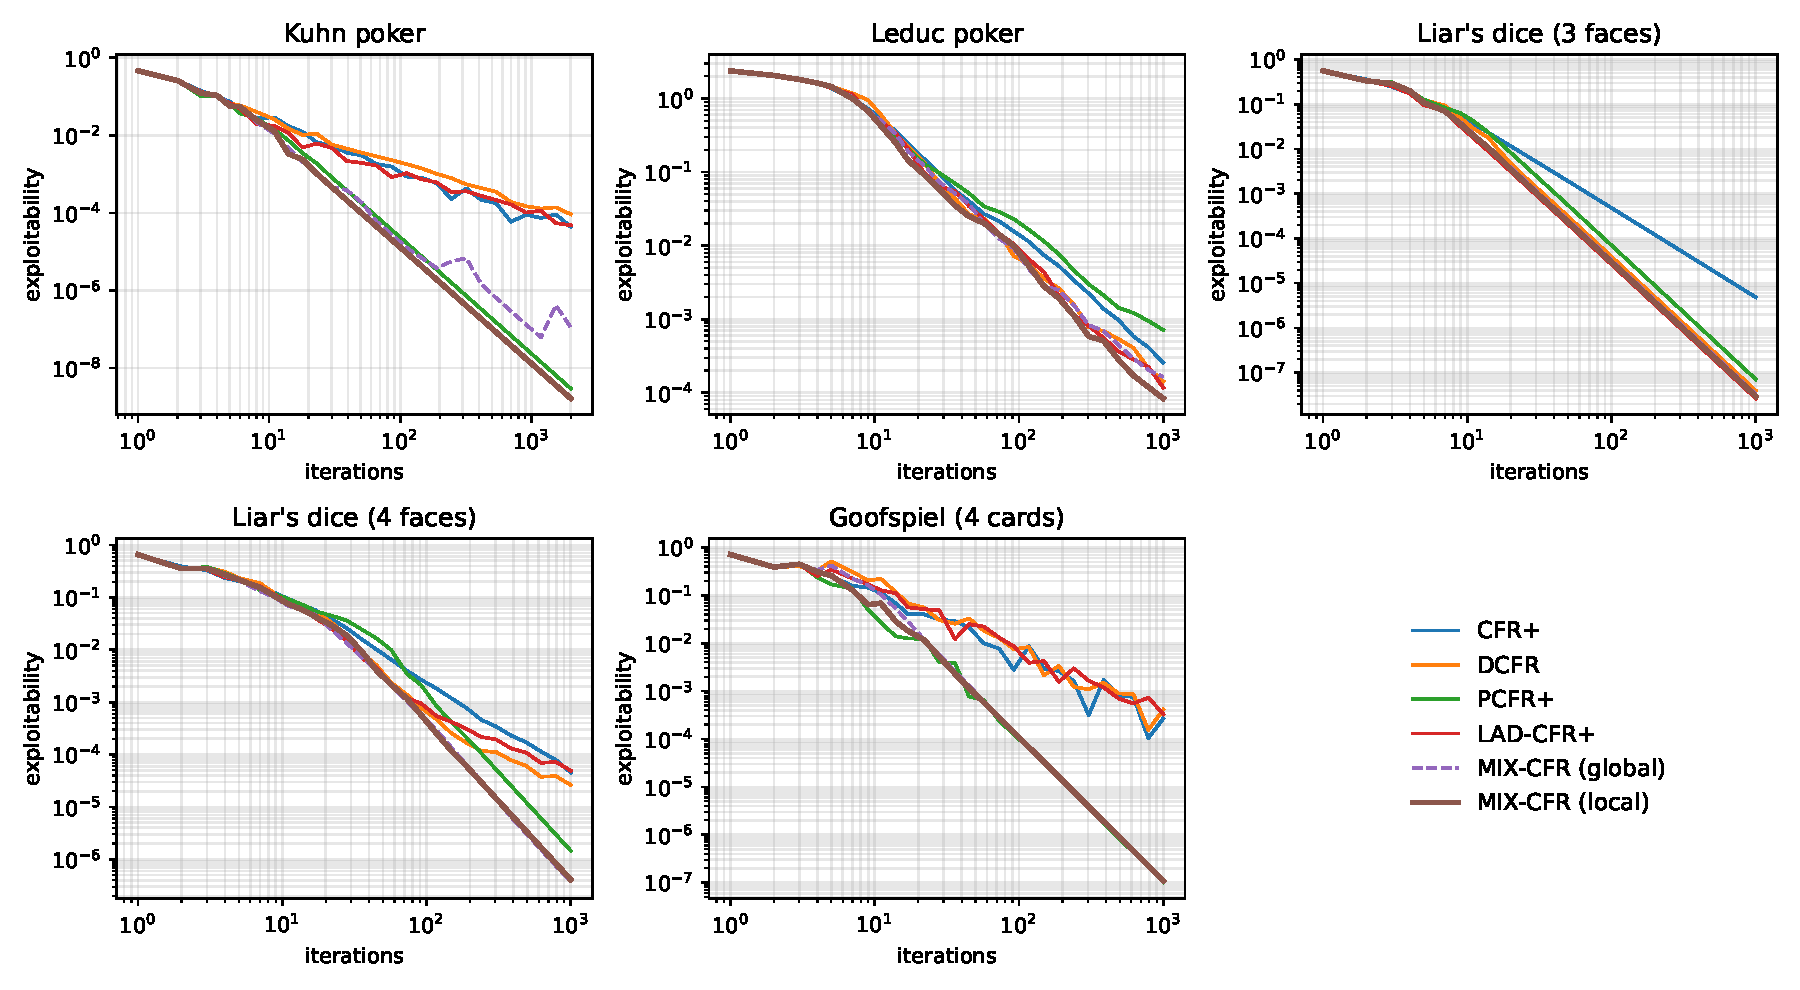
\includegraphics[width=0.92\textwidth]{figures/convergence.pdf}
\caption{Exploitability of the average strategy versus iterations (log--log). MIX-CFR
(local, thick line) is the best or close to the best method on every game, while each fixed
rule is clearly behind on at least one game.}
\label{fig:convergence}
\end{figure*}

\begin{table*}[t]
\centering
\caption{Exploitability after the final iteration (Table~\ref{tab:games}); lower is better,
best in bold. The best setting of \ours{} was selected on Kuhn and Leduc poker.}
\label{tab:main}
\begin{tabular}{@{}lcccccc@{}}
\toprule
\textbf{Game} & \textbf{\cfrp{}} & \textbf{DCFR} & \textbf{\pcfrp{}} & \textbf{\ours{}} &
\textbf{MIX-CFR (global)} & \textbf{MIX-CFR (local)} \\
\midrule
Kuhn poker           & $4.4\times10^{-5}$ & $9.2\times10^{-5}$ & $2.9\times10^{-9}$ & $4.8\times10^{-5}$ & $1.1\times10^{-7}$ & $\mathbf{1.6\times10^{-9}}$ \\
Leduc poker          & $2.6\times10^{-4}$ & $1.4\times10^{-4}$ & $7.1\times10^{-4}$ & $1.2\times10^{-4}$ & $1.6\times10^{-4}$ & $\mathbf{8.4\times10^{-5}}$ \\
Liar's dice (3)      & $4.8\times10^{-6}$ & $4.0\times10^{-8}$ & $7.1\times10^{-8}$ & $\mathbf{2.7\times10^{-8}}$ & $3.3\times10^{-8}$ & $3.0\times10^{-8}$ \\
Liar's dice (4)      & $4.5\times10^{-5}$ & $2.6\times10^{-5}$ & $1.5\times10^{-6}$ & $4.9\times10^{-5}$ & $\mathbf{3.7\times10^{-7}}$ & $4.1\times10^{-7}$ \\
Goofspiel (4)        & $2.7\times10^{-4}$ & $4.1\times10^{-4}$ & $\mathbf{1.0\times10^{-7}}$ & $3.3\times10^{-4}$ & $1.1\times10^{-7}$ & $1.1\times10^{-7}$ \\
\bottomrule
\end{tabular}
\end{table*}

\textbf{No fixed rule wins everywhere.} Table~\ref{tab:main} and Fig.~\ref{fig:convergence}
show that the ranking of the existing methods depends strongly on the game. \pcfrp{} is the
best fixed rule on Kuhn poker, Liar's dice with four faces and Goofspiel, but the worst method
on Leduc poker, where it is $2.8\times$ worse than \cfrp{}. DCFR is the best fixed rule on Leduc
poker but is worse than \cfrp{} on Kuhn poker and Goofspiel.

\textbf{MIX-CFR is consistently strong.} The local version of MIX-CFR is the best method on Kuhn
poker ($1.8\times$ lower exploitability than \pcfrp{}) and Leduc poker ($1.7\times$ lower than
DCFR, $3.1\times$ lower than \cfrp{}), and within $1.13\times$ of the best method on the other
three games. On Leduc poker and on Liar's dice with four faces, it is better than every
expert it combines: $3.6\times$ better than \pcfrp{} on the latter. It is the only method that is
not far behind the best on any game, and it achieves this without any tuning.

\textbf{Local versus global.} With the same experts, the local meta learner is $69\times$ better
than the global one on Kuhn poker and $2.0\times$ better on Leduc poker. It is slightly better on
Liar's dice with three faces, equal on Goofspiel, and $1.1\times$ worse on Liar's dice with four
faces. On Kuhn poker, the local learners give DCFR an average weight of $0.32$, compared with
$0.10$ for the global learner after 2000 iterations, which shows that information sets differ in which rule
suits them.

\textbf{Locally adaptive discounting.} Table~\ref{tab:lad} isolates the effect of the adaptive
discount. Compared with \cfrp{} using the same $t^2$ averaging, \ours{} lowers exploitability on
four of five games, including $1.8\times$ on Leduc poker. The local version is better than the
global version with the same settings on all five games. However, adapting only the discount
does not close the gap to the best fixed rule: \ours{} is worse than plain \cfrp{} on Liar's
dice with four faces and Goofspiel, and far behind \pcfrp{} on Kuhn poker and Goofspiel. Its
results were also sensitive to its settings. Discounting more strongly than DCFR at volatile
information sets increased exploitability by one to two orders of magnitude on both tuning
games.

\begin{table}[t]
\centering
\caption{Isolating the adaptive discount: exploitability of \cfrp{} variants with
$t^2$ averaging. ``Uniform'' applies the DCFR discount ($\alpha=3/2$) at every information set.}
\label{tab:lad}
\setlength{\tabcolsep}{3pt}
\begin{tabular}{@{}lcccc@{}}
\toprule
\textbf{Game} & \textbf{\cfrp{}} & \textbf{Uniform} & \textbf{\ours{} glob.} & \textbf{\ours{}} \\
\midrule
Kuhn         & $7.4\times10^{-5}$ & $4.8\times10^{-5}$ & $1.2\times10^{-4}$ & $\mathbf{4.8\times10^{-5}}$ \\
Leduc        & $2.1\times10^{-4}$ & $1.9\times10^{-4}$ & $1.4\times10^{-4}$ & $\mathbf{1.2\times10^{-4}}$ \\
Liar's d.\ (3) & $3.0\times10^{-8}$ & $3.9\times10^{-8}$ & $2.9\times10^{-8}$ & $\mathbf{2.7\times10^{-8}}$ \\
Liar's d.\ (4) & $4.5\times10^{-5}$ & $\mathbf{3.5\times10^{-5}}$ & $5.2\times10^{-5}$ & $4.9\times10^{-5}$ \\
Goofspiel    & $4.0\times10^{-4}$ & $\mathbf{1.1\times10^{-4}}$ & $5.6\times10^{-4}$ & $3.3\times10^{-4}$ \\
\bottomrule
\end{tabular}
\end{table}

\begin{table}[t]
\centering
\caption{MIX-CFR ablations: exploitability relative to the full method (values above 1 are
worse).}
\label{tab:ablation}
\setlength{\tabcolsep}{3pt}
\begin{tabular}{@{}lccccc@{}}
\toprule
\textbf{Variant} & \textbf{Kuhn} & \textbf{Leduc} & \textbf{LD(3)} & \textbf{LD(4)} & \textbf{Goof.} \\
\midrule
without \cfrp{}       & 866   & 2.20 & 1.23 & 0.90 & 24.2 \\
without DCFR          & 0.94  & 1.89 & 0.96 & 1.01 & 0.67 \\
without \pcfrp{}      & $3.7\times10^{4}$ & 1.49 & 1.01 & 30.9 & 2700 \\
predictive meta       & 1.13  & 1.41 & 1.00 & 1.05 & 29.7 \\
global meta           & 68.5  & 1.97 & 1.11 & 0.90 & 1.03 \\
\bottomrule
\end{tabular}
\end{table}

\textbf{Ablations.} Table~\ref{tab:ablation} shows that every expert matters somewhere.
Removing \pcfrp{} increases exploitability by factors of $31$ to $3.7\times10^{4}$ on Kuhn
poker, Liar's dice with four faces and Goofspiel, and removing \cfrp{} hurts on four of five games. DCFR is needed mainly on
Leduc poker, where removing it nearly doubles exploitability, which is the game where DCFR is
the best fixed rule. A predictive meta learner does not help and is $30\times$ worse on
Goofspiel, so we use plain regret matching$^+$.

\textbf{Cost.} MIX-CFR updates three experts per information set, but the tree traversal
dominates the running time. Its wall-clock time per run was between $0.9\times$ and
$1.5\times$ that of \cfrp{}. These timings were measured with eight runs in parallel on one
machine, so they are approximate.


\section{Discussion and Conclusion}
\label{sec:conclusion}

We asked whether adapting the CFR regret update to the local dynamics of each information set
improves convergence. Our results suggest that it does, but that \emph{what} is adapted
matters. Adapting only the discount on past regret (\ours{}) helped relative to \cfrp{} with the
same averaging, and its local version consistently beat its global version, which supports
the idea that information sets differ in how much past regret they should keep. However, its
gains were modest, depended on settings selected on the evaluation games, and did not
transfer to all held-out games. Letting each information set choose among existing update rules
(MIX-CFR) was much more effective. Without any tuning, it was the best or close to the best
method on all five games, while every fixed rule was far behind on at least one, and on two
games it outperformed all of the rules it combines.

\textbf{Limitations.} Our games are small enough for exact exploitability, and the runs are
limited to 1000--2000 iterations, so it remains open whether the advantage persists in much
larger games, in longer runs, or with sampling-based CFR. The local meta learner was clearly
better than the global one on Kuhn and Leduc poker but not on every game, so the benefit of
local selection also depends on the game. Our convergence guarantee covers the uniform average
strategy, not the $t^2$-weighted average used in the experiments. Finally, our timings come
from a Python implementation run in parallel and are approximate.

\textbf{Future work.} Natural extensions are adding more experts, such as PDCFR$^+$ or
APCFR$^+$, evaluating on larger games with a C++ implementation, and analyzing which features
of an information set determine the expert it selects.


\bibliographystyle{ieeetr}
\bibliography{ref}

\appendix
\section{Work Distribution}

Table~\ref{tab:work} summarizes each team member's contributions to this assignment.

\begin{table}[h]
\centering
\caption{Team member contributions.}
\label{tab:work}
\renewcommand{\arraystretch}{1.25}
\begin{tabular}{@{}p{0.2\columnwidth}p{0.36\columnwidth}p{0.36\columnwidth}@{}}
\toprule
\textbf{Area} & \textbf{Sadiqah Mushtaq} & \textbf{Umna Khawaja} \\
\midrule
Technical (reading background papers, presentations) & 50\% & 50\% \\
Coding (writing code) & 50\% & 50\% \\
Writing (paper writing) & 50\% & 50\% \\
\bottomrule
\end{tabular}
\end{table}


\end{document}
